\documentclass{beamer}
\usepackage[utf8]{inputenc}

\usetheme{Madrid}
\usecolortheme{default}
\usepackage{extarrows}
\usepackage{amsmath}
\usepackage{extarrows}
\usepackage{amssymb,amsfonts,amsthm}
\usepackage{txfonts}
\usepackage{tkz-euclide}
\usepackage{listings}
\usepackage{adjustbox}
\usepackage{array}
\usepackage{tabularx}
\usepackage{gvv}
\usepackage{lmodern}
\usepackage{circuitikz}
\usepackage{tikz}
\usepackage{graphicx}
\usepackage{amsmath} 

\setbeamertemplate{page number in head/foot}[totalframenumber]

\usepackage{tcolorbox}
\tcbuselibrary{minted,breakable,xparse,skins}

\definecolor{bg}{gray}{0.95}
\DeclareTCBListing{mintedbox}{O{}m!O{}}{%
  breakable=true,
  listing engine=minted,
  listing only,
  minted language=#2,
  minted style=default,
  minted options={%
    linenos,
    gobble=0,
    breaklines=true,
    breakafter=,,
    fontsize=\small,
    numbersep=8pt,
    #1},
  boxsep=0pt,
  left skip=0pt,
  right skip=0pt,
  left=25pt,
  right=0pt,
  top=3pt,
  bottom=3pt,
  arc=5pt,
  leftrule=0pt,
  rightrule=0pt,
  bottomrule=2pt,
  toprule=2pt,
  colback=bg,
  colframe=orange!70,
  enhanced,
  overlay={%
    \begin{tcbclipinterior}
    \fill[orange!20!white] (frame.south west) rectangle ([xshift=20pt]frame.north west);
    \end{tcbclipinterior}},
  #3,
}
\lstset{
    language=C,
    basicstyle=\ttfamily\small,
    keywordstyle=\color{blue},
    stringstyle=\color{orange},
    commentstyle=\color{green!60!black},
    numbers=left,
    numberstyle=\tiny\color{gray},
    breaklines=true,
    showstringspaces=false,
}
\title %optional
{10.6.4}

\author 
{EE25BTECH11049-Sai Krishna Bakki}

\begin{document}

\frame{\titlepage}
\begin{frame}{Question}
Draw a circle of radius 5cm. From a point 8cm away from its centre, construct a pair of tangents to the circle.
\end{frame}
\begin{frame}{Theoretical Solution}
    Let's take center as origin $\vec{O}$ and a point 8cm aways from its center as $\vec{h}=\myvec{8\\0}$.\\
The equation of a circle is given by 
\begin{align}
    g\brak{\vec{x}}=\norm{\vec{x}}^2+2\vec{u}^T\vec{x}+f=0
\end{align}
for
\begin{align}
\textbf{center}=\myvec{0\\0}, \text{since } \vec{c}=\vec{-u} 
\end{align}
we get
\begin{align}
\vec{u}=\myvec{0\\0}
\end{align}
we also know for any circle
\begin{align}
    \vec{V}=\myvec{1&0\\0&1}
\end{align}
\end{frame}
\begin{frame}
radius(r) = 5cm, we know that  $r^2=\norm{u}^2-f$ which gives us 
\begin{align}
    f=-25
\end{align}
By using below equation, we can determine the direction vectors of the tangent lines from an external point
\begin{align} \vec{m}^T\sbrak{\brak{\vec{V}\vec{h}+\vec{u}}\brak{\vec{V}\vec{h}+\vec{u}}^T-\vec{V}g\brak{\vec{h}}}\vec{m}=0\\
g\brak{h}=39
\label{eq:tangent}
\end{align}
where $\vec{m}=\myvec{m_x\\m_y}$ is the direction vectors of a tangent line.\\
Substituting values in $\eqref{eq:tangent}$, we get
\begin{align}
\myvec{m_x&m_y}\myvec{25&0\\0&-39}\myvec{m_x\\m_y}=0\\
25m_x^2-39m_y^2=0\\
\end{align}
The slopes of the tangent line is given by $k=\frac{d_x}{d_x}$. we solve for the slopes:
\end{frame}
\begin{frame}
\begin{align}
    k^2=\frac{25}{39}\implies k=\pm\frac{5}{\sqrt{39}}
\end{align}
Now, normal vectors of tangent lines are
\begin{align}
    \vec{n_1}=\myvec{5\\ \sqrt{39}},\vec{n_2}=\myvec{5\\ -\sqrt{39}}
\end{align}
Equations of tangent lines which passes through a point 8cm away from the center are
\begin{align}
    \vec{n_1^T}\vec{x}=c,\vec{n_2^T}\vec{x}=c
\end{align}
substituting $\vec{h}$ in line equation to get c,we get
\begin{align}
    c=40\\
    \myvec{5&\sqrt{39}}\vec{x}=40\\
    \myvec{5&-\sqrt{39}}\vec{x}=40
\end{align}
\end{frame}
\begin{frame}
Now, solve for points of contact, for that we use the following formulae
\begin{align}
    \vec{q_i}=\brak{\pm r\brak{\frac{\vec{n_i}}{\norm{\vec{n_i}}}}-\vec{u}}
\end{align}
we get
\begin{align}
    \vec{q_1}=\myvec{\frac{25}{8}\\\frac{5\sqrt{39}}{8}},
    \vec{q_2}=\myvec{\frac{25}{8}\\-\frac{5\sqrt{39}}{8}}
\end{align}
\end{frame}
\begin{frame}[fragile]
\frametitle{C Code}
\begin{lstlisting}
#include <stdio.h>
#include <math.h>

    // Define a simple structure for a 2D point.
    struct Point {
        double x;
        double y;
    };

    // This function calculates the two tangent points (t1, t2) for a circle
    // centered at the origin with a given radius 'r', from an external point 'p'.
    // The results are returned via pointers.
    void calculate_tangents(double r, struct Point p, struct Point* t1, struct Point* t2) {
        // 1. Calculate the x-coordinate of the polar line.
        // This is where the line connecting the tangent points intersects the x-axis.
\end{lstlisting}
\end{frame}
\begin{frame}[fragile]
\frametitle{C Code}
\begin{lstlisting}
        double x_contact = (r * r) / p.x;

        // 2. Use the circle equation (x^2 + y^2 = r^2) to find the y-coordinates.
        double y_contact_sq = (r * r) - (x_contact * x_contact);

        // If y_contact_sq is negative, the point is inside the circle, and no tangents exist.
        if (y_contact_sq < 0) {
            // Set coordinates to NaN (Not a Number) to indicate an error.
            t1->x = t1->y = NAN;
            t2->x = t2->y = NAN;
            return;
        }
double y_contact = sqrt(y_contact_sq);
// 3. Assign the coordinates to the output structures.
        t1->x = x_contact;
        t1->y = y_contact;
\end{lstlisting}
\end{frame}
\begin{frame}[fragile]
\frametitle{C Code}
\begin{lstlisting}
        t2->x = x_contact;
        t2->y = -y_contact;
    }
// Main function to demonstrate the tangent calculation for the specified problem.
    int main() {
        // Problem parameters: Circle radius 5, external point at (8, 0).
        double radius = 5.0;
        struct Point external_point = {8.0, 0.0};

        // Structures to hold the results.
        struct Point tangent_point1;
        struct Point tangent_point2;

        // Call the function to perform the calculation.
        calculate_tangents(radius, external_point, &tangent_point1, &tangent_point2);
\end{lstlisting}
\end{frame}
\begin{frame}[fragile]
\frametitle{C Code}
\begin{lstlisting}
        // Print the results.
        printf("Problem: Find tangents to a circle (radius=%.1f) from point (%.1f, %.1f)\n",
            radius, external_point.x, external_point.y);
        printf("----------------------------------------------------------------------\n");
        printf("Calculated Tangent Point 1 (T1): (%.4f, %.4f)\n", tangent_point1.x, tangent_point1.y);
        printf("Calculated Tangent Point 2 (T2): (%.4f, %.4f)\n", tangent_point2.x, tangent_point2.y);

        return 0;
    }  
\end{lstlisting}
\end{frame}
\begin{frame}[fragile]
\frametitle{Python Through Shared Output Code}
\begin{lstlisting}
import ctypes
import numpy as np
import matplotlib.pyplot as plt
import os

# --- C LIBRARY INTEGRATION ---

# Define a Python class that mirrors the C Point struct.
class Point(ctypes.Structure):
    _fields_ = [("x", ctypes.c_double),
                ("y", ctypes.c_double)]

# Load the shared C library.
# This assumes the compiled library is in the same directory.
lib_path = './circs.so'
if not os.path.exists(lib_path):
    print("Error: Shared library 'circs.so' not found.")
    print("Please compile the C code first with: gcc -shared -o libtangent.so -fPIC tangent_calc.c")
    \end{lstlisting}
\end{frame}
\begin{frame}[fragile]
\frametitle{Python Through Shared Output Code}
\begin{lstlisting}
else:
    tangent_lib = ctypes.CDLL(lib_path)

    # Define the function signature for the tangent calculation function.
    calculate_tangents_c = tangent_lib.calculate_tangents
    calculate_tangents_c.argtypes = [ctypes.c_double, Point, ctypes.POINTER(Point), ctypes.POINTER(Point)]
    calculate_tangents_c.restype = None

    # --- PROBLEM SETUP AND C FUNCTION CALL ---

    # 1. Define the problem: circle of radius 5, point 8cm away.
    circle_radius = 5.0
    external_point_p = Point(8.0, 0.0)

    # Create empty Point structures to hold the results from the C function.
    \end{lstlisting}
\end{frame}
\begin{frame}[fragile]
\frametitle{Python Through Shared Output Code}
\begin{lstlisting}
    tangent_point_t1 = Point()
    tangent_point_t2 = Point()

    # 2. Call the C function to perform the calculation.
    calculate_tangents_c(
        circle_radius,
        external_point_p,
        ctypes.byref(tangent_point_t1),
        ctypes.byref(tangent_point_t2)
    )

    # 3. Print the results calculated by the C code.
    print(f"Results from C function:")
    print(f"Tangent Point 1 (T1): ({tangent_point_t1.x:.4f}, {tangent_point_t1.y:.4f})")
    print(f"Tangent Point 2 (T2): ({tangent_point_t2.x:.4f}, {tangent_point_t2.y:.4f})")
# --- PLOTTING ---
# Helper function to generate circle points.
\end{lstlisting}
\end{frame}
\begin{frame}[fragile]
\frametitle{Python Through Shared Output Code}
\begin{lstlisting}
    def circ_gen(center, r):
        theta = np.linspace(0, 2 * np.pi, 100)
        x = center[0] + r * np.cos(theta)
        y = center[1] + r * np.sin(theta)
        return x, y

    # Generate circle for plotting.
    x_circ, y_circ = circ_gen([0, 0], circle_radius)

    # Plot the circle.
    plt.plot(x_circ, y_circ, label='Circle: $x^2 + y^2 = 25$')
    # Plot the key points.
    plt.scatter([0], [0], color='black', label='Center O(0,0)')
    plt.scatter([external_point_p.x], [external_point_p.y], color='red', label=f'External Point P({external_point_p.x:.0f}, {external_point_p.y:.0f})')
    plt.scatter([tangent_point_t1.x, tangent_point_t2.x], [tangent_point_t1.y, tangent_point_t2.y], color='green', label='Tangent Points')
\end{lstlisting}
\end{frame}
\begin{frame}[fragile]
\frametitle{Python Through Shared Output Code}
\begin{lstlisting}
    # Plot the tangent lines.
    plt.plot([external_point_p.x, tangent_point_t1.x], [external_point_p.y, tangent_point_t1.y], 'r--')
    plt.plot([external_point_p.x, tangent_point_t2.x], [external_point_p.y, tangent_point_t2.y], 'r--', label='Tangents')
    plt.text(tangent_point_t1.x + 0.5, tangent_point_t1.y, f'T1 ({tangent_point_t1.x:.2f}, {tangent_point_t1.y:.2f})')
    plt.text(tangent_point_t2.x + 0.5, tangent_point_t2.y - 0.5, f'T2 ({tangent_point_t2.x:.2f}, {tangent_point_t2.y:.2f})')
    plt.title('Construction of Tangents to a Circle (C + Python)')
    plt.xlabel('x-axis')
    plt.ylabel('y-axis')
    plt.gca().set_aspect('equal', adjustable='box')
    plt.grid(True)
    plt.legend()
    plt.show()
\end{lstlisting}
\end{frame}
\begin{frame}[fragile]
\frametitle{Python Code}
\begin{lstlisting}
import numpy as np
import matplotlib.pyplot as plt

# Helper function to generate points for a line segment
def line_gen(A, B):
    """Generates points for a line segment between A and B."""
    # Extend the line for better visualization by using a wider range
    len = 20
    x_AB = np.zeros((2, len))
    lam_1 = np.linspace(-0.5, 1.5, len) # Use a wider range to draw a longer line
    for i in range(len):
        temp1 = A + lam_1[i] * (B - A)
        x_AB[:, i] = temp1.flatten()
    return x_AB

# Helper function to generate points for a circle
def circ_gen(O, r):
\end{lstlisting}
\end{frame}
\begin{frame}[fragile]
\frametitle{Python Code}
\begin{lstlisting}
    """Generates points for a circle with center O and radius r."""
    len = 100
    theta = np.linspace(0, 2 * np.pi, len)
    x_circ = np.zeros((2, len))
    x_circ[0, :] = r * np.cos(theta)
    x_circ[1, :] = r * np.sin(theta)
    x_circ = (x_circ.T + O.flatten()).T
    return x_circ

# 1. DEFINE CIRCLE AND EXTERNAL POINT
# Circle parameters
O = np.array([[0], [0]]) # Center at origin
r = 5                     # Radius 5cm
# External point P (8cm from the center)
P = np.array([[8], [0]])

# 2. CALCULATE TANGENT POINTS
# The points of contact lie on the polar line x = r^2 / P_x
x_contact = r**2 / P[0, 0]
\end{lstlisting}
\end{frame}
\begin{frame}[fragile]
\frametitle{Python Code}
\begin{lstlisting}
# Find the y-coordinates by substituting x into the circle equation x^2 + y^2 = r^2
y_contact_sq = r**2 - x_contact**2
y_contact = np.sqrt(y_contact_sq)

# The two points of contact
T1 = np.array([[x_contact], [y_contact]])
T2 = np.array([[x_contact], [-y_contact]])

# 3. GENERATE GEOMETRIES FOR PLOTTING
# Generate the circle
x_circ = circ_gen(O, r)
# Generate the two tangent lines
x_tangent1 = line_gen(P, T1)
x_tangent2 = line_gen(P, T2)

# 4. PLOTTING
# Plot the tangent lines and the circle
\end{lstlisting}
\end{frame}
\begin{frame}[fragile]
\frametitle{Python Code}
\begin{lstlisting}
plt.plot(x_tangent1[0, :], x_tangent1[1, :], label='Tangent 1')
plt.plot(x_tangent2[0, :], x_tangent2[1, :], label='Tangent 2')
plt.plot(x_circ[0, :], x_circ[1, :], label='Circle')

# Plot the polar line
plt.axvline(x=x_contact, color='r', linestyle='--', label=f'Polar Line (x={x_contact:.2f})')

# Plot and label the key points
points = {'O (Center)': O, 'P (External Pt)': P, 'T1': T1, 'T2': T2}
for label, point in points.items():
    plt.scatter(point[0], point[1])
    plt.annotate(f'{label}\n({point[0,0]:.2f}, {point[1,0]:.2f})',
                 (point[0,0], point[1,0]),
                 textcoords="offset points",
                 xytext=(10,5),
                 ha='left')
\end{lstlisting}
\end{frame}
\begin{frame}[fragile]
\frametitle{Python Code}
\begin{lstlisting}
plt.text(0, 3, r'$x^2 + y^2 = 25$', fontsize=12, color='blue', ha='center')
plt.text(5.5, 2.5, r'$5x - \sqrt{39}y - 40 = 0$', fontsize=12, color='green', rotation=-32)
plt.text(5.5, -2.5, r'$5x + \sqrt{39}y - 40 = 0$', fontsize=12, color='purple', rotation=32)
# Set plot properties
ax = plt.gca()
ax.spines['left'].set_position('zero')
ax.spines['bottom'].set_position('zero')
ax.spines['right'].set_color('none')
ax.spines['top'].set_color('none')
plt.legend()
plt.grid(True)
plt.axis('equal')
plt.title('Construction of Tangents to a Circle')
plt.xlabel('x')
plt.ylabel('y')
plt.show()
\end{lstlisting}
\end{frame}
\begin{frame}{Plot By C code and Python Code}
    \begin{figure}
    \centering
    \caption{}
    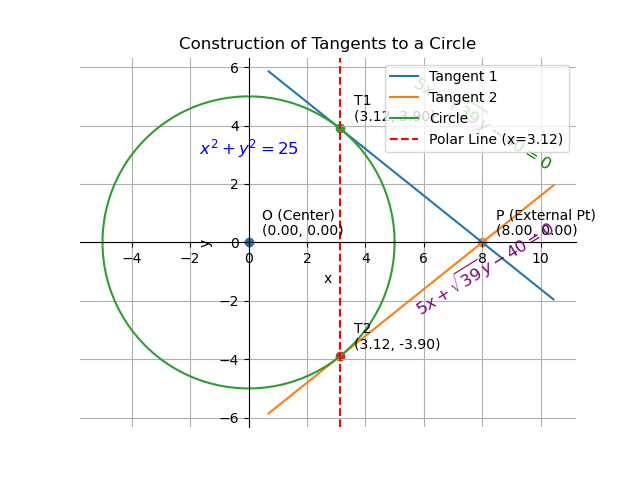
\includegraphics[width=0.7\columnwidth]{figs/Figure_1.png}
    \label{fig:placeholder}
\end{figure}
\end{frame}
\end{document}